\documentclass[12pt]{article}
\usepackage[paper=letterpaper,margin=2cm]{geometry}
\usepackage{amsmath,amssymb,amsfonts}
\usepackage{newtxtext, newtxmath}
\usepackage{enumitem}
\usepackage{titling}
\usepackage[colorlinks=true]{hyperref}

\usepackage{listings}
\usepackage[font=small,labelfont=bf]{caption} % Required for specifying captions to tables and figures

\usepackage{graphicx} % Required for the inclusion of images
\graphicspath{{./images/}} % Specifies the directory where pictures are stored

\setlength{\droptitle}{-6em}

\begin{document}

\center
Aprendizagem 2024\\
Homework I -- Group 016\\
(ist1106022, ist1106720)\vskip 1cm

\large{\textbf{Part I}: Pen and paper}\normalsize

\begin{enumerate}[leftmargin=\labelsep, label=\textbf{\arabic*.)}]
    \item ola
\end{enumerate}

\large{\textbf{Part II}: Programming}\normalsize

\begin{enumerate}[leftmargin=\labelsep, label=\textbf{\arabic*.)}]
    \item Applying \texttt{f\_classif} from the \texttt{sklearn} library upon the dataset (after splitting into feature data matrix and target vector) allows understanding of the discrimantive power of each feature: \vskip 0.25cm
          \begin{lstlisting}[basicstyle=\ttfamily\centering]
'Pregnancies': 39.67
'Glucose': 213.16
'BloodPressure': 3.26
'SkinThickness': 4.3
'Insulin': 13.28
'BMI': 71.77
'DiabetesPedigreeFunction': 23.87
'Age': 46.14
        \end{lstlisting}
          The scores indicate that \texttt{Glucose} is the \textbf{most discriminative} feature, whereas \texttt{BloodPressure} is the \textbf{least discriminative}.
          The following plot shows the class-condition probability density functions for these two features:\vskip 0.25cm
          \begin{center}
              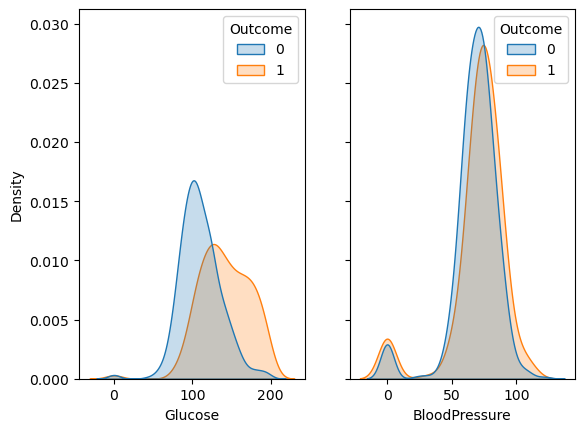
\includegraphics{discrimantive_features_dense_probability.png}
          \end{center}
    \item To measure accuracy levels originated from using a decision tree with the minimums sample split values (2, 5, 10, 20, 30, 50, 100) when branching, a stratified 80-20 training-testing split was performed. \\ \vspace{0.25em} Additionally, since \texttt{sklearn} performs non-deterministic thresholding of numeric variables in decision trees, the results were made by averaging over 10 runs per parametrization (leading to the error margins in the graph). \\ \vspace{0.25em} The following graph shows the different averaged accuracy levels for the decision tree classifiers generated for each minimum split: \\
          \begin{center}
              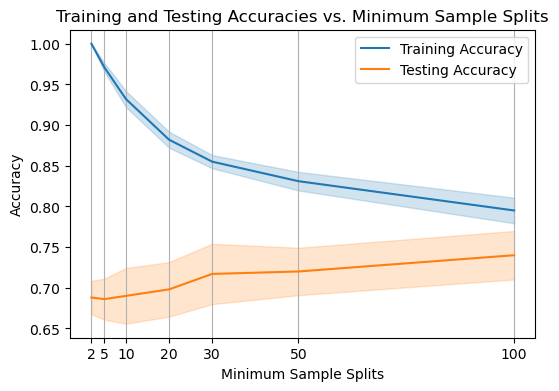
\includegraphics{split_training_results.png}
          \end{center}
    \item The smaller decision tree minimum splits have the highest accuracy levels on the training set, while having the smaller values on the testing set, which indicates overfitting.
          The following minimum splits lead to increansigly better accuracy values on the testing set, although continuing to decrease the accuracy on the training set, which indicates the model is starting to have better generalization capabilities and less overfitting. \\\vspace{0.25em}
          Out of all the available minimum splits, the best pick would be the one leading to a smaller difference in accuracies between the two sets, which in this case would be 100. \\\vspace{0.25em}
          Ideally with higher minimum sample split values, there would be a value leading high and identical accuracy levels on both sets.
    \item \begin{enumerate}[label=\textbf{\roman*.)}]
              \item Using \textit{all} data to train a single decision tree classifier with a maximum depth of 3 leads to the following tree (\texttt{value} and \texttt{samples} expressed in proportion):\\
                    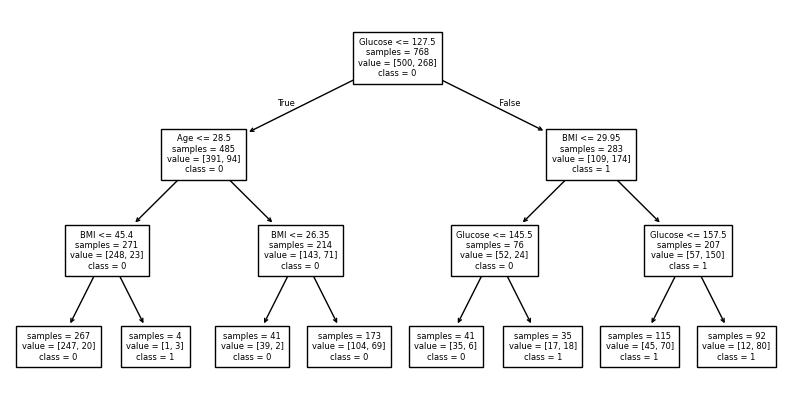
\includegraphics{decision_tree_value_counts.png}\\
                    \vspace{2em}
                    But with this second view of the same tree, we can more easily understand the probability of each class in each node:\\
                    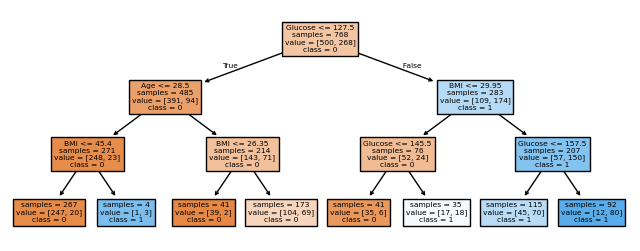
\includegraphics{decision_tree.png} \\
                    The \textcolor{orange}{"oranger"} the node, the higher the probability of the class being 0 (eq. non-diabetic), and the \textcolor{blue}{"bluer"} the node, the higher the probability of the class being 1 (eq. diabetic). \\
              \item Overall, high \texttt{Glucose} and \texttt{BMI} are the most common indicator of diabetes. (agreeing with our analysis in \textit{exercise 1}). \\\vspace{0.25em}
                    Following is a thorough analysis of the probability in each conditional association (extracted from the graph):
                    \vspace{0.5em}
                    \begin{itemize}
                        \item $P( \text{\texttt{Diabetes}}) = 0.349$
                    \end{itemize}
                    \begin{itemize}
                        \item $P( \text{\texttt{Diabetes | Glucose $\leq 127.5$}}) = 0.194$:
                              \begin{itemize}
                                  \item $P( \text{\texttt{Diabetes | Glucose $\leq 127.5$ \& Age $\leq 28.5$}}) = 0.085$:
                                        \begin{itemize}
                                            \item $P( \text{\texttt{Diabetes | Glucose $\leq 127.5$ \& Age $\leq 28.5$ \& BMI $\leq 45.4$}}) = 0.075$
                                            \item $P( \text{\texttt{Diabetes | Glucose $\leq 127.5$ \& Age $\leq 28.5$ \& BMI $> 45.4$}}) = 0.75$
                                        \end{itemize}
                                  \item $P( \text{\texttt{Diabetes | Glucose $\leq 127.5$ \& Age $> 28.5$}}) = 0.332$:
                                        \begin{itemize}
                                            \item $P( \text{\texttt{Diabetes | Glucose $\leq 127.5$ \& Age $> 28.5$ \& BMI $\leq 26.35$}}) = 0.049$
                                            \item $P( \text{\texttt{Diabetes | Glucose $\leq 127.5$ \& Age $> 28.5$ \& BMI $> 26.35$}}) = 0.399$
                                        \end{itemize}
                              \end{itemize}
                    \end{itemize}
                    \begin{itemize}
                        \item $P( \text{\texttt{Diabetes | Glucose $> 127.5$}}) = 0.615$:
                              \begin{itemize}
                                  \item $P( \text{\texttt{Diabetes | Glucose $> 127.5$ \& BMI $\leq 29.95$}}) = 0.316$:
                                        \begin{itemize}
                                            \item $P( \text{\texttt{Diabetes | Glucose $> 127.5$ \& BMI $\leq 29.95$ \& Glucose $\leq 145.5$}}) = 0.146$
                                            \item $P( \text{\texttt{Diabetes | Glucose $> 127.5$ \& BMI $\leq 29.95$ \& Glucose $> 145.5$}}) = 0.514$
                                        \end{itemize}
                                  \item $P( \text{\texttt{Diabetes | Glucose $> 127.5$ \& BMI $> 29.95$}}) = 0.725$:
                                        \begin{itemize}
                                            \item $P( \text{\texttt{Diabetes | Glucose $> 127.5$ \& BMI $> 29.95$ \& Glucose $\leq 157.5$}}) = 0.609$
                                            \item $P( \text{\texttt{Diabetes | Glucose $> 127.5$ \& BMI $> 29.95$ \& Glucose $> 157.5$}}) = 0.87$
                                        \end{itemize}
                              \end{itemize}
                    \end{itemize}
                    \vspace{0.5em}
                    From the analysis it is possible to easily understand the likelihood of a new patient, given his retrieved medical data, to have diabetes or not.
          \end{enumerate}
\end{enumerate}
\end{document}
